% Chapter 7: Regularization for Deep Learning

\chapter{Regularization for Deep Learning}
\label{chap:regularization}

This chapter explores techniques to improve generalization and prevent overfitting in deep neural networks. Regularization helps models perform well on unseen data.


\begin{learningobjectives}
\objective{Why regularization is needed and how it improves generalization}
\objective{Norm penalties (L1, L2, Elastic Net) and identify when to use each}
\objective{Data augmentation strategies across vision, text, and audio tasks}
\objective{Early stopping and understand its interaction with optimization}
\objective{Dropout and normalization layers and reason about their effects}
\objective{Advanced techniques such as label smoothing, mixup, adversarial training, and gradient clipping}
\end{learningobjectives}




% Chapter 7, Section 1

\section{Parameter Norm Penalties \difficultyInline{intermediate}}
\label{sec:parameter-penalties}

\textbf{Parameter norm penalties} constrain model capacity by penalizing large weights.

\subsection{Intuition: Shrinking the Model's "Complexity"}

Think of a model as a musical band with many instruments (parameters). If every instrument plays loudly (large weights), the result can be noisy and overfit to the training song. Norm penalties are like asking the band to lower the volume uniformly (L2) or mute many instruments entirely (L1) so the melody (true signal) stands out. This discourages memorization and encourages simpler patterns that generalize.

\subsection{L2 Regularization (Weight Decay)}

Add squared L2 norm of weights to the loss:

\begin{equation}
\tilde{L}(\vect{\theta}) = L(\vect{\theta}) + \frac{\lambda}{2} \|\vect{w}\|^2
\end{equation}

Gradient update becomes:
\begin{equation}
\vect{w} \leftarrow (1 - \alpha\lambda)\vect{w} - \alpha \nabla_{\vect{w}} L
\end{equation}

The factor $(1 - \alpha\lambda)$ causes "weight decay."

\subsection{L1 Regularization}

L1 regularization adds the L1 norm of weights to the loss function: $\tilde{L}(\vect{\theta}) = L(\vect{\theta}) + \lambda \|\vect{w}\|_1$. L1 regularization promotes sparsity by driving many weights to become exactly zero, making it useful for feature selection where only the most important features are retained. The gradient of L1 regularization is $\text{sign}(\vect{w})$, which provides a constant magnitude update that encourages weights to move toward zero, effectively performing automatic feature selection by eliminating less important parameters.

% Index entries
\index{regularization!L2}
\index{regularization!L1}
\index{elastic net}

\subsection{Elastic Net}

Combines L1 and L2:
\begin{equation}
\tilde{L}(\vect{\theta}) = L(\vect{\theta}) + \lambda_1 \|\vect{w}\|_1 + \lambda_2 \|\vect{w}\|^2
\end{equation}


% Chapter 7, Section 2

\section{Dataset Augmentation \difficultyInline{intermediate}}
\label{sec:data-augmentation}

\textbf{Data augmentation} artificially increases training set size by applying transformations that preserve labels.

\subsection{Intuition: Seeing the Same Thing in Many Ways}

Humans recognize an object despite different viewpoints, lighting, or small occlusions. Augmentation teaches models the same robustness by showing multiple, label-preserving variations of each example. This reduces overfitting by making spurious correlations less useful and forcing the model to focus on invariant structure.

\subsection{Image Augmentation}

Image augmentation employs various transformations to artificially expand the training dataset while preserving semantic content. Geometric transformations including rotation, translation, scaling, flipping, and cropping change the spatial properties of images while preserving the semantic content, where rotation and translation help models become invariant to object orientation and position, while scaling and cropping teach robustness to different object sizes and partial views. Color modifications such as brightness, contrast, and saturation adjustments simulate different lighting conditions and camera settings that occur in real-world scenarios, where by varying these color properties, models learn to focus on structural features rather than specific color characteristics, improving generalization across different environments. Noise augmentation including Gaussian noise and blur helps models become more robust to sensor imperfections and motion blur that occur in real images, where this regularization technique prevents overfitting to pixel-perfect training data and improves performance on noisy real-world inputs. Cutout and erasing techniques randomly remove rectangular regions from images, forcing the model to learn from partial information and encouraging the network to not rely on specific spatial locations, instead learning more distributed, robust feature representations. Mixup creates new training examples by linearly interpolating between pairs of images and their corresponding labels, encouraging smoother decision boundaries and reducing overconfident predictions, leading to better calibration and generalization.

Example: horizontal flip
\begin{equation}
\vect{x}_{\text{aug}} = \text{flip}(\vect{x}), \quad y_{\text{aug}} = y
\end{equation}

\subsection{Text Augmentation}

Text augmentation techniques for natural language processing include synonym replacement, which replaces words with their synonyms while preserving the original meaning and label, helping models become more robust to vocabulary variations and reducing overfitting to specific word choices, improving generalization to unseen text variations. Random insertion and deletion operations randomly add or remove words from sentences, simulating natural language variations and typos, where this augmentation helps models become more robust to noisy text inputs and teaches them to focus on important content rather than exact word sequences. Back-translation translates text to another language and then back to the original language, creating paraphrased versions with the same meaning, generating diverse sentence structures while preserving semantic content and helping models learn more robust language representations. Paraphrasing rewrites sentences using different wording while maintaining the same meaning and label, exposing models to various ways of expressing the same concept and improving their ability to generalize to different writing styles and linguistic variations.

\subsection{Audio Augmentation}

Audio augmentation techniques for speech and audio processing include time stretching, which changes the duration of audio signals without affecting pitch, simulating different speaking rates and helping models become robust to variations in speech tempo while preserving the fundamental frequency characteristics and semantic content of the audio. Pitch shifting modifies the fundamental frequency of audio while keeping the duration constant, simulating different voice characteristics and helping models learn pitch-invariant features while improving generalization across speakers with different vocal ranges. Adding background noise introduces various types of noise to simulate real-world acoustic environments, helping models become robust to environmental factors like room acoustics, background conversations, and equipment noise, improving performance in noisy conditions. SpecAugment randomly masks frequency bands or time segments in spectrograms, forcing models to learn from partial information and encouraging the network to develop more robust acoustic representations that don't rely on specific frequency or temporal patterns.

\begin{figure}[htbp]
\centering
\begin{tikzpicture}
    % Original image placeholder
    \draw[fill=bookpurple!10] (0,0) rectangle (3,2);
    \node at (1.5,1) {Original};
    % Rotated
    \begin{scope}[xshift=120]
        \draw[fill=bookpurple!10,rotate=10] (0,0) rectangle (3,2);
        \node at (1.5,1) {Rotate};
    \end{scope}
    % Flipped
    \begin{scope}[xshift=240]
        \draw[fill=bookpurple!10] (0,0) rectangle (3,2);
        \node at (1.5,1) {Flip};
    \end{scope}
    % Cropped
    \begin{scope}[yshift=-80]
        \draw[fill=bookpurple!10] (0,0) rectangle (3,2);
        \draw[bookred,thick] (0.5,0.5) rectangle (2.5,1.5);
        \node at (1.5,1) {Crop};
    \end{scope}
    % Color jitter
    \begin{scope}[xshift=120,yshift=-80]
        \shade[left color=bookpurple!10,right color=bookred!20] (0,0) rectangle (3,2);
        \node at (1.5,1) {Color};
    \end{scope}
    % Cutout
    \begin{scope}[xshift=240,yshift=-80]
        \draw[fill=bookpurple!10] (0,0) rectangle (3,2);
        \draw[fill=bookblack!60] (1,0.7) rectangle (2,1.3);
        \node at (1.5,1) {Cutout};
    \end{scope}
\end{tikzpicture}
\caption{Illustration of common image augmentations. Variants preserve labels while encouraging invariances.}
\label{fig:augmentation-examples}
\end{figure}

% Index entries
\index{data augmentation}
\index{augmentation!vision}
\index{augmentation!text}
\index{augmentation!audio}


% Chapter 7, Section 3

\section{Early Stopping \difficultyInline{intermediate}}
\label{sec:early-stopping}

\textbf{Early stopping} monitors validation performance and stops training when it begins to degrade.

\subsection{Intuition: Stop Before You Memorize}

Imagine studying for an exam. Initially, practice improves your understanding (training and validation improve). If you keep cramming the exact same questions, you start memorizing answers that don't help with new questions (training improves, validation worsens). Early stopping is the principle of stopping at the point of best validation performance to avoid memorization.

\subsection{Algorithm}

\begin{enumerate}
    \item Train model and evaluate on validation set periodically
    \item Track best validation performance
    \item If no improvement for $p$ epochs (patience), stop
    \item Return model with best validation performance
\end{enumerate}

\begin{algorithm}[Early stopping meta-algorithm]
Let $n$ be the number of steps between evaluations.\\
Let $p$ be the patience (number of worsened validations before stopping).\\
Let $\vect{\theta}_0$ be the initial parameters.

\begin{enumerate}[leftmargin=*]
    \item $\vect{\theta} \leftarrow \vect{\theta}_0$, $i \leftarrow 0$, $j \leftarrow 0$, $v \leftarrow \infty$
    \item $\vect{\theta}^* \leftarrow \vect{\theta}$, $i^* \leftarrow i$
    \item \textbf{while} $j < p$ \textbf{do}
    \begin{enumerate}
        \item Update $\vect{\theta}$ by running the training algorithm for $n$ steps
        \item $i \leftarrow i + n$
        \item $v' \leftarrow \text{ValidationSetError}(\vect{\theta})$
        \item \textbf{if} $v' < v$ \textbf{then}
        \begin{enumerate}
            \item $j \leftarrow 0$
            \item $\vect{\theta}^* \leftarrow \vect{\theta}$, $i^* \leftarrow i$, $v \leftarrow v'$
        \end{enumerate}
        \item \textbf{else} $j \leftarrow j + 1$
        \item \textbf{end if}
    \end{enumerate}
    \item \textbf{end while}
    \item Return best parameters $\vect{\theta}^*$ and best step $i^*$
\end{enumerate}
\end{algorithm}

\subsection{Benefits}

\begin{itemize}
    \item \textbf{Simple and effective:} Requires only tracking validation performance and a patience parameter; widely used in practice \cite{GoodfellowEtAl2016,Prince2023}.
    \item \textbf{Automatically determines training duration:} Finds a good stopping time without a pre-fixed epoch budget, often saving substantial compute.
    \item \textbf{Implicit regularization:} Halting before convergence limits effective capacity by keeping weights smaller and preventing memorization; in some regimes it mimics an L2 constraint under gradient descent \cite{GoodfellowEtAl2016}.
    \item \textbf{Compatible with many settings:} Works with any loss, architecture (MLPs, CNNs, Transformers), and optimizer.
    \item \textbf{Reduces computational cost:} Training stops as soon as overfitting begins, reducing energy/time.
    \item \textbf{Improves generalization stability:} Curbs validation variance late in training when overfitting spikes.
\end{itemize}

\subsection{Considerations}

\begin{itemize}
    \item \textbf{Validation protocol:} Requires a reliable validation set and evaluation cadence; noisy metrics may trigger premature stops. Use smoothing or require monotone improvements.
    \item \textbf{Patience and frequency:} Patience $p$ and evaluation interval $n$ interact with LR schedules; too small $p$ can stop before a scheduled LR drop helps.
    \item \textbf{Checkpointing:} Always restore the best model (not the last); keep track of the weights at the best validation step.
    \item \textbf{Warmup and plateaus:} With warmup or long plateaus, consider larger patience or metric smoothing.
    \item \textbf{Multi-metric objectives:} For tasks with multiple metrics (e.g., accuracy and calibration), pick the primary metric or a composite.
    \item \textbf{Distributed training:} Ensure validation statistics are aggregated consistently across devices to avoid spurious decisions.
    \item \textbf{Historical context:} Early stopping predates modern deep learning and was popular in classical neural nets and boosting as a strong regularizer; it remains a standard baseline \cite{GoodfellowEtAl2016,Bishop2006}.
\end{itemize}

\begin{example}
\textbf{Example (vision):} Train a ResNet on CIFAR-10 with validation accuracy checked each epoch; use patience $p=20$. Accuracy peaks at epoch 142; training halts at 162 without improvement, and the checkpoint from 142 is used for testing.
\end{example}

\begin{figure}[htbp]
\centering
\begin{tikzpicture}[scale=0.85]
    % axes
    \draw[->] (0,0) -- (9,0) node[right] {Epochs};
    \draw[->] (0,0) -- (0,4.5) node[above] {Loss};
    % training loss curve
    \draw[draw=bookred, thick] plot[smooth] coordinates {(0.3,4) (1,3.2) (2,2.6) (3,2.2) (4,1.9) (5,1.7) (6,1.5) (7,1.4) (8,1.35)};
    % validation loss curve (U-shaped)
    \draw[draw=bookpurple, thick] plot[smooth] coordinates {(0.3,3.9) (1,3.1) (2,2.5) (3,2.15) (4,1.95) (5,1.92) (6,1.95) (7,2.05) (8,2.2)};
    % vertical line at best epoch
    \draw[dashed] (4,0) -- (4,4.5) node[above] {Best epoch};
    \node[text=bookpurple] at (6.9,2.3) {Validation};
    \node[text=bookred] at (7.3,1.35) {Training};
\end{tikzpicture}
\caption{Early stopping: validation loss reaches a minimum before training loss; the best checkpoint is saved and restored.}
\label{fig:early-stopping-curve}
\end{figure}

% Index entries
\index{early stopping}
\index{validation set}


% Chapter 7, Section 4

\section{Dropout \difficultyInline{intermediate}}
\label{sec:dropout}

\textbf{Dropout} randomly deactivates neurons during training, preventing co-adaptation.

\subsection{Intuition: Training a Robust Ensemble}

Dropout is like asking different subsets of a team to work on the same task on different days. No single member can rely on a particular colleague always being present, so each learns to be broadly useful. This results in a robust team (model) that performs well even when some members (neurons) are inactive.

\subsection{Training with Dropout}

Training with dropout involves sampling a binary mask $\vect{m}$ with $P(m_i = 1) = p$ for each layer at each training step, then applying the mask to the activations: $\vect{h} = \vect{m} \odot \vect{h}$. Mathematically, this is expressed as $\vect{h}_{\text{dropout}} = \vect{m} \odot f(\mat{W}\vect{x} + \vect{b})$ where $m_i \sim \text{Bernoulli}(p)$, effectively randomly deactivating neurons with probability $1-p$ during training to prevent co-adaptation and improve generalization.

\begin{figure}[htbp]
\centering
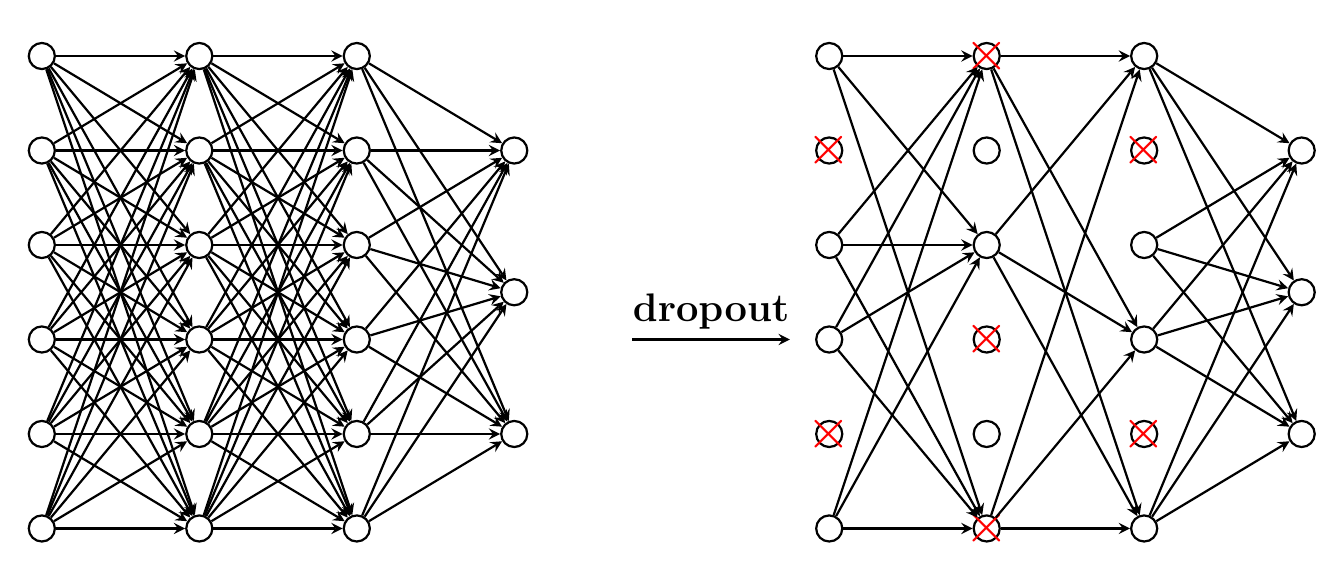
\begin{tikzpicture}[
    node/.style={circle, draw, thick},
  ]

\def\layersep{2}
\def\nodesep{1.2}

  % Input layer (6 nodes)
  \foreach \y in {1,...,6}{
      \node[node] (i\y) at (0,\nodesep*\y) {};
    }

  % Hidden layer 1 (6 nodes)
  \foreach \y in {1,...,6}{
      \node[node] (h1\y) at (\layersep,\nodesep*\y) {};
    }

  % Hidden layer 2 (6 nodes)
  \foreach \y in {1,...,6}{
      \node[node] (h2\y) at (2*\layersep,\nodesep*\y) {};
    }

  % Output layer (3 nodes)
  \node[node] (o1) at (3*\layersep,\nodesep*2) {};
  \node[node] (o2) at (3*\layersep,\nodesep*3.5) {};
  \node[node] (o3) at (3*\layersep,\nodesep*5) {};

  % Connections
  \foreach \source in {1,...,6}
  \foreach \dest in {1,...,6}{
      \path[-stealth, thick] (i\source) edge (h1\dest);
      \path[-stealth, thick] (h1\source) edge (h2\dest);
    }
  \foreach \source in {1,...,6}
  \foreach \dest in {1,2,3}
  \draw[-stealth, thick] (h2\source) -- (o\dest);

  % Dropout arrow
  \draw[-stealth, thick] (7.5,3*\nodesep) -- node[above,font=\Large\bfseries] {dropout} (9.5, 3*\nodesep);

  % After dropout - Input layer (6 nodes, drop 2)
  \foreach \y in {1,...,6}
  \node[node] (di\y) at (10,\nodesep*\y) {};

  \node[red,font=\huge] at (di2) {$\times$};
  \node[red,font=\huge] at (di5) {$\times$};

  % After dropout - Hidden layer 1 (6 nodes, drop 3)
  \foreach \y in {1,...,6}
  \node[node] (dh1\y) at (10+\layersep,\nodesep*\y) {};

  \node[red,font=\huge] at (dh11) {$\times$};
  \node[red,font=\huge] at (dh13) {$\times$};
  \node[red,font=\huge] at (dh16) {$\times$};

  % After dropout - Hidden layer 2 (6 nodes, drop 2)
  \foreach \y in {1,...,6}
  \node[node] (dh2\y) at (10+2*\layersep,\nodesep*\y) {};

  \node[red,font=\huge] at (dh22) {$\times$};
  \node[red,font=\huge] at (dh25) {$\times$};

  % After dropout - Output layer (3 nodes)
  \node[node] (do1) at (10+3*\layersep,\nodesep*2) {};
  \node[node] (do2) at (10+3*\layersep,\nodesep*3.5) {};
  \node[node] (do3) at (10+3*\layersep,\nodesep*5) {};

  % After dropout connections
  \foreach \source in {1,3,4,6}
  \foreach \dest in {1,4,6}
  \draw[-stealth, thick] (di\source) -- (dh1\dest);

  \foreach \source in {1,4,6}
  \foreach \dest in {1,3,6}
  \draw[-stealth, thick] (dh1\source) -- (dh2\dest);

  \foreach \source in {1,3,4,6}
  \foreach \dest in {1,2,3}
  \draw[-stealth, thick] (dh2\source) -- (do\dest);

\end{tikzpicture}
\caption{Dropout training process: randomly deactivating neurons (marked with $\times$) creates different subnetworks during each training step, forcing the network to learn robust representations that don't rely on specific neurons.}
\label{fig:dropout-training-process}
\end{figure}

\subsection{Inference}

At test time, scale outputs by dropout probability:
\begin{equation}
\vect{h}_{\text{test}} = p \cdot f(\mat{W}\vect{x} + \vect{b})
\end{equation}

Or equivalently, scale weights during training by $\frac{1}{p}$ (inverted dropout).

In practice, modern frameworks implement \emph{inverted dropout}: during training, activations are scaled by $\tfrac{1}{p}$ after masking so that the expected activation matches test-time activations, and no scaling is needed at inference \cite{Srivastava2014,GoodfellowEtAl2016}. For convolutional layers, use the same $p$ per feature map to avoid distribution shift.

\subsection{Interpretation}

Dropout can be viewed as an implicit ensemble where sampling masks trains an ensemble of $2^n$ subnetworks whose shared weights yield a form of model averaging. It also acts as noise injection where multiplicative Bernoulli noise on activations provides data-dependent regularization analogous to adding Gaussian noise for linear models. Additionally, dropout relates to approximate Bayesian inference where with appropriate priors, it connects to variational inference, and applying dropout at test time with multiple passes (MC dropout) estimates predictive uncertainty, making it useful for uncertainty quantification in safety-critical applications.

\begin{example}
\textbf{Example (uncertainty):} Run $T=20$ stochastic forward passes with dropout enabled at test time and average predictions to obtain mean and variance; high variance flags low-confidence inputs.
\end{example}

\subsection{Variants}

DropConnect drops individual weights instead of activations, promoting sparsity at the parameter level and providing a different form of regularization. Spatial Dropout drops entire feature maps in CNNs to preserve spatial coherence and regularize channel reliance, which is particularly useful for convolutional layers. Variational Dropout uses the same dropout mask across time steps in RNNs to avoid injecting different noise per step that can harm temporal consistency, making it more suitable for sequential data. MC Dropout keeps dropout active at inference and averages predictions to quantify epistemic uncertainty, which is useful in safety-critical applications where uncertainty estimation is crucial. Concrete and Alpha Dropout provide continuous relaxations or distributions tailored for specific activations like SELU to maintain self-normalizing properties, offering more sophisticated regularization approaches for specific network architectures.

\begin{figure}[htbp]
\centering
\begin{tikzpicture}[scale=0.9]
    % simple schematic: three subnetworks averaged
    \node[draw, rectangle, fill=bookpurple!15] (s1) at (0,0) {Subnetwork 1};
    \node[draw, rectangle, fill=bookpurple!15] (s2) at (3,0) {Subnetwork 2};
    \node[draw, rectangle, fill=bookpurple!15] (s3) at (6,0) {Subnetwork 3};
    \node[draw, circle, fill=bookpurple!20] (avg) at (3,-1.8) {Average};
    \draw[->] (s1) -- (avg);
    \draw[->] (s2) -- (avg);
    \draw[->] (s3) -- (avg);
\end{tikzpicture}
\caption{Dropout as implicit model averaging over many subnetworks.}
\label{fig:dropout-ensemble}
\end{figure}

\begin{figure}[htbp]
\centering
\begin{tikzpicture}[scale=0.9]
    % Layer nodes
    \foreach \i in {1,2,3}
        \node[circle, draw, fill=bookpurple!15, minimum size=0.7cm] (x\i) at (0,-\i) {};
    \foreach \i in {1,2,3,4}
        \node[circle, draw, fill=bookpurple!25, minimum size=0.7cm] (h\i) at (2,-\i*0.8) {};
    \foreach \i in {1,2}
        \node[circle, draw, fill=bookred!15, minimum size=0.7cm] (y\i) at (4,-\i) {};

    % Full connections (light color)
    \foreach \i in {1,2,3}
        \foreach \j in {1,2,3,4}
            \draw[->,bookpurple!30] (x\i) -- (h\j);
    \foreach \i in {1,2,3,4}
        \foreach \j in {1,2}
            \draw[->,bookpurple!30] (h\i) -- (y\j);

    % Dropped neurons (crossed)
    \draw[bookred, line width=1.2pt] (h2) ++(-0.25,-0.25) -- ++(0.5,0.5);
    \draw[bookred, line width=1.2pt] (h2) ++(0.25,-0.25) -- ++(-0.5,0.5);
    \draw[bookred, line width=1.2pt] (h4) ++(-0.25,-0.25) -- ++(0.5,0.5);
    \draw[bookred, line width=1.2pt] (h4) ++(0.25,-0.25) -- ++(-0.5,0.5);

    \node at (2,0.5) {\small Randomly dropped (training)};
\end{tikzpicture}
\caption{Dropout during training: randomly deactivating hidden units encourages redundancy and robustness.}
\label{fig:dropout-diagram}
\end{figure}

% Index entries
\index{dropout}
\index{regularization!dropout}


% Chapter 7, Section 5

\section{Batch Normalization \difficultyInline{intermediate}}
\label{sec:batch-normalization}

\textbf{Batch normalization} normalizes layer inputs across the batch dimension.

\subsection{Intuition: Keeping Scales Stable}

Training can become unstable if the distribution of activations shifts as earlier layers update (internal covariate shift). Batch normalization re-centers and re-scales activations, keeping them in a predictable range so downstream layers see a more stable input distribution. This allows larger learning rates and speeds up training.

\subsection{Algorithm}

For mini-batch $\mathcal{B}$ with activations $\vect{x}$:

\begin{align}
\mu_{\mathcal{B}} &= \frac{1}{|\mathcal{B}|} \sum_{i \in \mathcal{B}} x_i \\
\sigma^2_{\mathcal{B}} &= \frac{1}{|\mathcal{B}|} \sum_{i \in \mathcal{B}} (x_i - \mu_{\mathcal{B}})^2 \\
\hat{x}_i &= \frac{x_i - \mu_{\mathcal{B}}}{\sqrt{\sigma^2_{\mathcal{B}} + \epsilon}} \\
y_i &= \gamma \hat{x}_i + \beta
\end{align}

where $\gamma$ and $\beta$ are learnable parameters.

Implementation details: maintain running averages $\mu_{\text{running}}, \sigma^2_{\text{running}}$ updated with momentum $\rho$ per iteration; apply per-feature normalization for fully connected layers and per-channel per-spatial-location statistics for CNNs \cite{Ioffe2015,GoodfellowEtAl2016}.

\subsection{Benefits}

\begin{itemize}
    \item \textbf{Stabilizes distributions:} Mitigates internal covariate shift, keeping activations in a stable range \cite{Ioffe2015}.
    \item \textbf{Enables larger learning rates:} Better-conditioned optimization allows faster training.
    \item \textbf{Less sensitive initialization:} Wider set of workable initializations \cite{GoodfellowEtAl2016}.
    \item \textbf{Regularization effect:} Mini-batch noise in statistics acts as stochastic regularization, improving generalization.
    \item \textbf{Supports deeper nets:} Facilitates training very deep architectures (e.g., ResNets) \cite{He2016}.
    \item \textbf{Improves gradient flow:} Normalized scales yield healthier signal-to-noise ratios in backprop.
\end{itemize}

\subsection{Inference}

At test time, use running averages computed during training:
\begin{equation}
y = \gamma \frac{x - \mu_{\text{running}}}{\sqrt{\sigma^2_{\text{running}} + \epsilon}} + \beta
\end{equation}

Be careful when batch sizes are small at inference or differ from training: do not recompute batch statistics at test time; use the stored running averages. For distribution shift, consider recalibrating $\mu_{\text{running}}, \sigma^2_{\text{running}}$ with a small unlabeled buffer.

\subsection{Variants}

\textbf{Layer Normalization:} Normalize across features for each sample; effective in RNNs and Transformers where batch statistics are less stable.

\textbf{Group Normalization:} Normalize within groups of channels; robust to small batch sizes common in detection/segmentation.

\textbf{Instance Normalization:} Normalize each sample independently; prominent in style transfer where contrast/style per instance varies.

\textbf{Batch Renormalization / Ghost BatchNorm:} Adjust for mismatch between batch and population statistics or simulate small batches inside large ones for regularization.

\begin{example}
\textbf{Example (vision):} In a CNN with batch size 128, use per-channel BN after each convolution with momentum $\rho=0.9$ and $\epsilon=10^{-5}$. During inference, freeze $\gamma,\beta$ and use stored running statistics.
\end{example}

% Index entries
\index{batch normalization}
\index{normalization layers}
\index{internal covariate shift}


% Chapter 7, Section 6

\section{Other Regularization Techniques \difficultyInline{intermediate}}
\label{sec:other-regularization}

\subsection{Intuition: Many Small Guards Against Overfitting}

Beyond penalties and normalization, there are practical techniques that act like small guards during training. Each introduces a mild constraint or noise that nudges the model away from brittle solutions and encourages smoother decision boundaries.

\subsection{Label Smoothing}

Replace hard targets with smoothed distributions:
\begin{equation}
y'_k = (1 - \epsilon) y_k + \frac{\epsilon}{K}
\end{equation}

Prevents overconfident predictions and improves calibration by discouraging saturated logits; commonly used in large-scale classification (e.g., ImageNet) and sequence models. Choose $\epsilon$ in $[0.05, 0.2]$ depending on class count $K$ and desired calibration. It can also mitigate overfitting to annotator noise.

\begin{example}
\textbf{Example (ImageNet):} With $K=1000$ and $\epsilon=0.1$, the target for the correct class becomes $0.9$ while others receive $0.0001$ each; top-1 accuracy and ECE often improve.
\end{example}

\subsection{Gradient Clipping}

Limit gradient magnitude to prevent exploding gradients:

\begin{definition}[Clipping by Value]
Clipping by value limits each gradient component individually:
\begin{equation}
g \leftarrow \max(\min(g, \theta), -\theta)
\end{equation}
where $\theta$ is the clipping threshold. This method constrains each gradient element to lie within $[-\theta, \theta]$, providing component-wise control over gradient magnitudes.
\end{definition}

\begin{definition}[Clipping by Norm]
Clipping by norm rescales the entire gradient vector when its norm exceeds a threshold:
\begin{equation}
g \leftarrow \frac{g}{\max(1, \|g\| / \theta)}
\end{equation}
where $\theta$ is the clipping threshold. This method preserves the gradient direction while scaling its magnitude, making it preferred over value clipping as it maintains the relative importance of different parameters.
\end{definition}

Clipping stabilizes training in RNNs and very deep nets by preventing exploding gradients, especially with large learning rates or noisy batches. Norm clipping with threshold $\theta$ is preferred as it preserves direction while scaling magnitude. Excessive clipping can bias updates and slow convergence; tune $\theta$ w.r.t. optimizer and batch size.

\begin{example}
\textbf{Example (NLP):} Train a GRU with global norm clip $\theta=1.0$; without clipping, gradients occasionally explode causing loss spikes.
\end{example}
\begin{equation}
g \leftarrow \frac{g}{\max(1, \|g\| / \theta)}
\end{equation}

\subsection{Stochastic Depth}

Randomly skip residual blocks during training with survival probability $p_l$ per layer $l$, while using the full network depth at test time. This shortens expected depth during training, improving gradient flow and reducing overfitting in very deep networks \cite{Huang2016StochasticDepth}.

Let $p_l$ decrease with depth (e.g., linearly from 1.0 to $p_{\min}$). During training, with probability $1-p_l$ a residual block is bypassed; otherwise it is applied and its output is scaled to match test-time expectation.

\begin{example}
\textbf{Example (ResNets):} In a 110-layer ResNet, set $p_l$ from 1.0 to 0.8 across depth; training converges faster and generalizes better on CIFAR-10.
\end{example}

\subsection{Mixup}

Train on convex combinations of examples:
\begin{align}
\tilde{\vect{x}} &= \lambda \vect{x}_i + (1-\lambda) \vect{x}_j \\
\tilde{y} &= \lambda y_i + (1-\lambda) y_j
\end{align}

where $\lambda \sim \text{Beta}(\alpha, \alpha)$ and $\text{Beta}(\alpha, \alpha)$ is the Beta distribution with shape parameters $\alpha$ and $\alpha$, which controls the mixing strength and distribution of the interpolation weights.

Mixup encourages linear behavior between classes, reduces memorization of spurious correlations, and improves robustness to label noise \cite{Zhang2018Mixup}. Typical $\alpha$ values are in $[0.2, 1.0]$. Variants include CutMix (patch-level mixing) \cite{Yun2019CutMix} and Manifold Mixup (mix at hidden layers).

\begin{example}
\textbf{Example (vision):} With $\alpha=0.4$, randomly pair images in a batch and form convex combinations; train using the mixed targets. Improves top-1 accuracy and calibration.
\end{example}

\subsection{Adversarial Training}

Add adversarially perturbed examples to training:
\begin{equation}
\vect{x}_{\text{adv}} = \vect{x} + \epsilon \cdot \text{sign}(\nabla_{\vect{x}} L(\vect{x}, y))
\end{equation}

This FGSM objective can be extended to multi-step PGD adversaries. Adversarial training improves worst-case robustness but often reduces clean accuracy and increases compute \cite{Goodfellow2014}. Robust features learned can transfer across tasks; careful tuning of $\epsilon$, steps, and randomness is crucial.

\begin{example}
\textbf{Example (robust CIFAR-10):} Use $\epsilon=8/255$, $k=7$ PGD steps, step size $2/255$; train with a 1:1 mix of clean and adversarial samples.
\end{example}

\begin{remark}[Historical Context and Applications]
Label smoothing and dropout popularized regularization at scale; gradient clipping stabilized early RNNs; stochastic depth enabled training very deep residual networks; mixup and CutMix improved data-efficient generalization; adversarial training established the modern paradigm for robustness. Applications span medical imaging, autonomous driving, speech recognition, and large-scale language models where calibration and robustness are critical \cite{GoodfellowEtAl2016,He2016,Ioffe2015}.
\end{remark}

% Index entries
\index{label smoothing}
\index{gradient clipping}
\index{stochastic depth}
\index{mixup}
\index{adversarial training}


% Chapter 7: Real World Applications

\section{Real World Applications}
\label{sec:regularization-real-world}


Regularization techniques are essential for making deep learning models work reliably in real-world scenarios where data is messy and models need to perform well on new, unseen examples.

\subsection{Autonomous Vehicle Safety}

Self-driving cars rely heavily on regularization to ensure safe operation, where robust object detection uses regularization techniques like dropout and data augmentation to help vehicles recognize pedestrians, cyclists, and other vehicles under diverse conditions including rain, fog, night driving, and unusual angles, preventing system failures when encountering weather or lighting conditions not heavily represented in training data. Generalization to new environments is crucial, as a self-driving car trained in sunny California needs to work safely in snowy Boston, where regularization prevents the model from memorizing specific training locations and instead learns general driving principles that transfer across different cities and climates. Regularization helps prevent overfitting to rare events by maintaining good performance on common scenarios like normal traffic while still being prepared for rare but critical situations such as emergency vehicles and unexpected obstacles.

\subsection{Medical Imaging Analysis}

Healthcare applications use regularization to make reliable diagnoses, where cancer detection from limited data benefits from regularization techniques like data augmentation and early stopping that allow models to learn effectively from hundreds rather than millions of examples, making them practical for clinical use since medical datasets are often small because annotating medical images requires expert radiologists. Consistent performance across hospitals is achieved through regularization, where different hospitals use different imaging equipment, and regularization ensures models trained at one hospital generalize to work at others despite variations in image quality, resolution, or equipment manufacturers. Regularization helps reduce false positives in medical diagnosis, where false alarms cause unnecessary anxiety and costly follow-up tests, and techniques like label smoothing help models be appropriately confident, reducing overconfident but incorrect predictions.

\subsection{Natural Language Processing for Customer Service}

Chatbots and virtual assistants benefit from regularization, where handling diverse customer queries is improved through regularization techniques like data augmentation including paraphrasing and synonym replacement that help chatbots understand intent even when people use unexpected wording, since customers phrase questions in countless ways. Regularization prevents memorization of training conversations, where without regularization, chatbots might memorize training examples and give nonsensical responses to new queries, but dropout and other techniques force the model to learn general conversation patterns rather than specific exchanges. Regularization helps models adapt to evolving language, where language changes constantly with new slang and terminology, and regularization helps models stay flexible and adapt to linguistic shifts without extensive retraining.

\subsection{Key Benefits in Practice}

Regularization provides crucial advantages in real applications, where it works with limited data since not every problem has millions of training examples, reduces maintenance costs by helping models generalize better and requiring less frequent retraining, increases reliability by ensuring systems work consistently even when deployed conditions differ from training, and enables deployment by making models trustworthy enough for safety-critical applications. These examples show that regularization isn't just a mathematical nicety—it's the difference between models that work only in labs and those that succeed in the real world, where the techniques discussed in this chapter are essential for bridging the gap between theoretical deep learning and practical applications.

% Index entries
\index{applications!autonomous vehicles}
\index{applications!medical imaging}
\index{applications!chatbots}
\index{regularization!applications}

% % Chapter 7, Section 7

% \section{Exercises \difficultyInline{intermediate}}
% \label{sec:ch7-exercises}

% This section provides exercises to reinforce your understanding of regularization techniques. Exercises are categorized by difficulty and include hints.

% \subsection{Easy Exercises (6 exercises)}

% \begin{problem}[Identify Regularization]
% List whether each technique primarily reduces variance, bias, or both: L2, L1, dropout, data augmentation, early stopping, batch normalization.

% \textbf{Hint:} Consider effect on model capacity and training dynamics.
% \end{problem}

% \begin{problem}[Weight Decay Update]
% Given learning rate $\alpha$ and L2 coefficient $\lambda$, write the update rule for weights with gradient $g$.

% \textbf{Hint:} Combine gradient step with multiplicative shrinkage.
% \end{problem}

% \begin{problem}[L1 vs L2]
% Explain when L1 is preferred over L2, and vice versa.

% \textbf{Hint:} Sparsity, feature selection, stability, and correlated features.
% \end{problem}

% \begin{problem}[Early Stopping Curve]
% Sketch training and validation loss over epochs showing overfitting and stopping point.

% \textbf{Hint:} Validation loss reaches minimum before training loss.
% \end{problem}

% \begin{problem}[Augmentation Invariance]
% For image classification, list three invariances augmentation can teach and one risk.

% \textbf{Hint:} Rotation/translation invariance vs. label leakage or distribution shift.
% \end{problem}

% \begin{problem}[BatchNorm Inference]
% Explain why running averages are used at test time for batch normalization.

% \textbf{Hint:} Mini-batch statistics are noisy and unavailable at inference.
% \end{problem}

% \subsection{Medium Exercises (5 exercises)}

% \begin{problem}[Elastic Net Penalty]
% Derive the gradient of $\lambda_1 \|\vect{w}\|_1 + \frac{\lambda_2}{2}\|\vect{w}\|_2^2$ with respect to $\vect{w}$.

% \textbf{Hint:} Subgradient for L1; standard gradient for L2.
% \end{problem}

% \begin{problem}[Dropout Scaling]
% Show equivalence between scaling activations at test time by $p$ and scaling at training by $1/p$ (inverted dropout).

% \textbf{Hint:} Match expected activations across train/test.
% \end{problem}

% \begin{problem}[Early Stopping as Regularization]
% Argue how early stopping can mimic an L2 constraint under gradient descent.

% \textbf{Hint:} Consider that weights remain small when training halts early.
% \end{problem}

% \begin{problem}[Label Smoothing and Confidence]
% For $\epsilon>0$, show how label smoothing affects cross-entropy gradients.

% \textbf{Hint:} Replace one-hot $y$ by $(1-\epsilon)\,y + \epsilon/K$.
% \end{problem}

% \begin{problem}[Mixup Geometry]
% Explain how mixup encourages linear behavior between classes in representation space.

% \textbf{Hint:} Consider convex combinations and linear decision boundaries.
% \end{problem}

% \subsection{Hard Exercises (5 exercises)}

% \begin{problem}[Generalization Bound Intuition]
% Discuss how norm constraints relate to capacity control (e.g., Rademacher complexity) and generalization.

% \textbf{Hint:} Smaller norms can reduce hypothesis class complexity.
% \end{problem}

% \begin{problem}[Adversarial Training Trade-offs]
% Analyze how adversarial training affects robustness, clean accuracy, and optimization.

% \textbf{Hint:} Robust features vs. gradient masking and compute cost.
% \end{problem}

% \begin{problem}[BatchNorm and Optimization]
% Provide a theoretical or empirical argument for why batch normalization enables higher learning rates.

% \textbf{Hint:} Consider conditioning of the optimization problem.
% \end{problem}

% \begin{problem}[Stochastic Depth in Deep Nets]
% Model the expected depth under stochastic depth and discuss gradient flow implications.

% \textbf{Hint:} Consider per-layer survival probabilities.
% \end{problem}

% \begin{problem}[Design a Regularization Suite]
% Given a 100-class image dataset with 50k images, design a regularization suite (penalties, augmentation, normalization, schedules). Justify choices.

% \textbf{Hint:} Balance data, model size, compute budget, and desired robustness.
% \end{problem}

% % Index entries
% \index{exercises!regularization}
% \index{exercises!regularization}




% Chapter summary and problems
% Key Takeaways for Chapter 7

\section*{Key Takeaways}
\addcontentsline{toc}{section}{Key Takeaways}

\begin{keytakeaways}
\begin{itemize}[leftmargin=2em]
    \item \textbf{Regularisation} constrains model capacity to improve generalisation and prevent overfitting to training data.
    \item \textbf{Norm penalties} (L1, L2) encourage simpler models; L1 induces sparsity whilst L2 shrinks weights uniformly.
    \item \textbf{Data augmentation} artificially expands training sets by applying semantics-preserving transformations.
    \item \textbf{Dropout} randomly drops units during training, forcing redundant representations and reducing co-adaptation.
    \item \textbf{Early stopping and batch normalisation} are simple yet powerful techniques for better training dynamics and generalisation.
\end{itemize}
\end{keytakeaways}



% Exercises (Hands-On Exercises) for Chapter 7: Regularization for Deep Learning

\section*{Exercises}
\addcontentsline{toc}{section}{Exercises}

\subsection*{Easy}

\begin{exercisebox}[easy]
\begin{problem}[L1 vs L2 Regularisation]
Explain the difference between L1 and L2 regularisation. Which one is more likely to produce sparse weights, and why?
\end{problem}
\begin{hintbox}
Consider the shape of the L1 and L2 penalty terms and their gradients.
\end{hintbox}
\end{exercisebox}


\begin{exercisebox}[easy]
\begin{problem}[Data Augmentation Strategies]
List three common data augmentation techniques for image classification tasks and explain how each helps improve generalisation.
\end{problem}
\begin{hintbox}
Think about geometric transformations, colour adjustments, and realistic variations.
\end{hintbox}
\end{exercisebox}


\begin{exercisebox}[easy]
\begin{problem}[Early Stopping]
Describe how early stopping works as a regularisation technique. What metric should you monitor, and when should you stop training?
\end{problem}
\begin{hintbox}
Consider validation set performance and the risk of overfitting to the training set.
\end{hintbox}
\end{exercisebox}


\begin{exercisebox}[easy]
\begin{problem}[Dropout Interpretation]
During training, dropout randomly sets activations to zero with probability $p$. During inference, all neurons are active but their outputs are scaled. Explain why this scaling is necessary.
\end{problem}
\begin{hintbox}
Think about the expected value of activations during training versus inference.
\end{hintbox}
\end{exercisebox}


\subsection*{Medium}

\begin{exercisebox}[medium]
\begin{problem}[Regularisation Trade-off]
Given a model with both L2 regularisation and dropout, discuss how you would tune the regularisation strength $\lambda$ and dropout rate $p$. What signs would indicate too much or too little regularisation?
\end{problem}
\begin{hintbox}
Monitor training and validation loss curves, and consider the bias-variance trade-off.
\end{hintbox}
\end{exercisebox}


\begin{exercisebox}[medium]
\begin{problem}[Batch Normalisation Effect]
Explain how batch normalisation acts as a regulariser. Discuss its interaction with dropout.
\end{problem}
\begin{hintbox}
Consider the noise introduced by computing statistics on mini-batches and why dropout is often not needed with batch normalisation.
\end{hintbox}
\end{exercisebox}


\subsection*{Hard}

\begin{exercisebox}[hard]
\begin{problem}[Mixup Derivation]
Mixup trains on convex combinations of examples: $\tilde{\vect{x}} = \lambda \vect{x}_i + (1-\lambda)\vect{x}_j$ where $\lambda \sim \text{Beta}(\alpha, \alpha)$. Derive how this affects the decision boundary and explain why it improves generalisation.
\end{problem}
\begin{hintbox}
Consider the effect on the loss surface and the implicit regularisation from interpolating between examples.
\end{hintbox}
\end{exercisebox}


\begin{exercisebox}[hard]
\begin{problem}[Adversarial Training]
Design an adversarial training procedure for a classification model. Explain how to generate adversarial examples using FGSM (Fast Gradient Sign Method) and why this improves robustness.
\end{problem}
\begin{hintbox}
Adversarial examples are $\vect{x}_{adv} = \vect{x} + \epsilon \cdot \text{sign}(\nabla_{\vect{x}} L)$. Discuss the trade-off between clean and adversarial accuracy.
\end{hintbox}
\end{exercisebox}


\begin{exercisebox}[hard]
\begin{problem}[Early Stopping Strategy]
Explain how early stopping works as a regularisation technique. How do you determine the optimal stopping point?
\end{problem}
\begin{hintbox}
Monitor validation loss and stop when it starts increasing, indicating overfitting.
\end{hintbox}
\end{exercisebox}


\begin{exercisebox}[hard]
\begin{problem}[Data Augmentation Effects]
Compare different data augmentation techniques for image classification. Which techniques are most effective for different types of images?
\end{problem}
\begin{hintbox}
Consider geometric transformations, color jittering, and mixup techniques.
\end{hintbox}
\end{exercisebox}


\begin{exercisebox}[hard]
\begin{problem}[Weight Decay vs Dropout]
Compare the effects of weight decay and dropout regularisation. When would you use one over the other?
\end{problem}
\begin{hintbox}
Weight decay penalises large weights globally, while dropout creates sparse activations locally.
\end{hintbox}
\end{exercisebox}


\begin{exercisebox}[hard]
\begin{problem}[Batch Normalization vs Layer Normalization]
Compare batch normalisation and layer normalisation. When is each more appropriate?
\end{problem}
\begin{hintbox}
Batch normalisation depends on batch statistics, while layer normalisation is independent of batch size.
\end{hintbox}
\end{exercisebox}


\begin{exercisebox}[hard]
\begin{problem}[Regularisation in Convolutional Networks]
Explain how regularisation techniques differ when applied to convolutional layers versus fully connected layers.
\end{problem}
\begin{hintbox}
Consider spatial structure preservation and parameter sharing in convolutional layers.
\end{hintbox}
\end{exercisebox}


\begin{exercisebox}[hard]
\begin{problem}[Ensemble Regularisation]
How can ensemble methods be viewed as a form of regularisation? Compare bagging and boosting approaches.
\end{problem}
\begin{hintbox}
Ensembles reduce variance by averaging predictions from multiple models.
\end{hintbox}
\end{exercisebox}



